\chapter{Equilibrio termodinamico}
L'entropia di un sistema isolato è massima nel suo stato di equilibrio. Il sistema termodinamico è composto da un numero $N$ di componenti e le quantità termodinamiche rappresentano valori medi. Sono possibili quindi piccole fluttuazioni in tali valori. Da tali fluttuazioni l'entropia deve decrescere, altrimenti il sistema evolverebbe in un nuovo stato di equilibrio e quello precedente non sarebbe stabile. Da questo si possono dedurre importanti condizioni di equilibrio locale e di stabilità.
\begin{obs}
    Per semplicità, nel seguito ci si limita a considerare le coppie di variabili $(T,S)$, $(p,V)$ e $(\mu,N)$.
\end{obs}

\section{Equilibrio locale}
Si consideri un sistema isolato con $E$, $V$ ed $N$ fissati che si trovi in uno stato di equilibrio. Si supponga che in tale stato il sistema sia suddiviso in due parti $1$ e $2$ tali che 
\begin{equation}
    E = E_1 + E_2,\quad V = V_1 + V_2,\quad N = N_1 + N_2.
\end{equation}
Le due parti in cui è diviso il sistema possono essere ad esempio di un liquido oppure di una fase liquida in contatto con il suo vapore. La divisione in due parti può essere ideale o essere una parete mobile, induttiva e porosa. Si supponga ora che avvengano delle fluttuazioni spontanee $E_\alpha$, $V_\alpha$ ed $N_\alpha$ con i vincoli
\begin{equation}
\label{eq: vincoli variazioni sistema in due parti}
    \Delta E_2 = -\Delta E_1,\quad \Delta V_2 = -\Delta V_1,\quad \Delta N_2 = -\Delta N_1.
\end{equation}
Si assuma che le fluttuazioni siano piccole, in questo modo si può espandere al primo ordine il cambiamento di entropia dovuto a tali fluttuazioni
\begin{equation}
    \Delta S \simeq \sum_{\alpha = 1}^2\bigg[\frac{\p S}{\p E_\alpha}\bigg|_{V_\alpha,N_\alpha}^{eq}\Delta E_\alpha + \frac{\p S}{\p V_\alpha}\bigg|_{E_\alpha,N_\alpha}^{eq}\Delta V_\alpha + \frac{\p S}{\p N_\alpha}\bigg|_{E_\alpha,V_\alpha}^{eq}\Delta N_\alpha\bigg].
\end{equation}
Usando le equazioni di stato \eqref{eq: equazioni di stato da S} e le relazioni \eqref{eq: vincoli variazioni sistema in due parti} si ha
\begin{equation}
    \Delta S \simeq \bigg(\frac{1}{T_1^{eq}} - \frac{1}{T_2^{eq}}\bigg)\Delta E_1 + \bigg(\frac{p_1^{eq}}{T_1^{eq}} - \frac{p_2^{eq}}{T_2^{eq}}\bigg)\Delta V_1 - \bigg(\frac{\mu_1^{eq}}{T_1^{eq}} - \frac{\mu_2^{eq}}{T_2^{eq}}\bigg)\Delta N_1.
\end{equation}
Necessariamente, si deve avere $\Delta S \le 0$, ma $\Delta E_1$, $\Delta V_1$ e $\Delta N_1$ possono essere sia positivi che negativi, pertanto l'unico modo per non avere $\Delta S > 0$ è che siano vere
\begin{equation}
\label{eq: equilibrio termico sistema in due parti}
    T_1^{eq} = T_2^{{eq}},\quad p_1^{eq} = p_2^{eq},\quad \mu_1^{eq} = \mu_2^{eq},
\end{equation}
ovvero che il sistema sia in uno stato di equilibrio termico, meccanico e chimico tra le due parti. Inevitabilmente, si ha $\Delta S = 0$ al primo ordine nelle fluttuazioni. La discussione appena fatta per un sistema diviso in due parti può essere estesa ad un sistema diviso in $n$ parti richiedendo che le relazioni di equilibrio \eqref{eq: equilibrio termico sistema in due parti} siano valide per ognuna delle $n$ parti.

La condizione di equilibrio è sempre che $S$ sia massima, qualsiasi sia l'insieme di variabili di controllo scelte. A seconda di questo, la condizione di equilibrio può venire espressa come condizione di minimo per il potenziale di approccio. Ad esempio, per considerare le fluttuazioni di ripartizionamento di un sistema con $S$, $V$ e $N$ fissati, si può utilizzare l'energia interna $E(S, V, N)$ e richiedere che $\Delta E > 0$ per qualsiasi fluttuazione in queste condizioni. Con una trattazione del tutto analoga a quella fatta per $S(E, V, N)$ si trovano gli stessi risultati. All'equilibrio è necessario che siano verificate le equazioni \eqref{eq: equilibrio termico sistema in due parti} e che al primo ordine si abbia $\Delta E = 0$. Nell'analizzare i vincoli che emergono considerando il secondo ordine nelle piccoli fluttuazioni si è soliti sfruttare l'approccio in termini dei potenziali.

\subsection{Regola generale per i criteri di stabilità}
Si supponga che l'insieme delle variabili di controllo sia 
\begin{equation}
    \{X_1,\dots,X_{r},I_{r+1},\dots,I_n\},
\end{equation}
con le $X_i$ variabili estensive e le $I_j$ variabili intensive. Sia assuma inoltre che $\Phi(X_1,\dots,X_{r},I_{r+1},\dots,I_n)$ sia il potenziale appropriato, il cui differenziale è dato da
\begin{equation}
    d\Phi = \sum_{i = 1}^rI_idX_i - \sum_{j = r + 1}^nX_jdI_j.
\end{equation}
Lo stato di equilibrio è un minimo di $\Phi$, per cui per ogni fluttuazione si deve avere $\Delta\Phi \ge 0$. Si consideri quindi un partizionamento delle variabili estensive, ossia fluttuazioni tali che
\begin{equation}
    \delta X_i = \delta X_{i,1} + \delta X_{i,2} = 0.
\end{equation}
Al primo ordine nelle fluttuazioni si ha allora
\begin{equation}
    \Delta\Phi^{(1)} = \nsum_i\bigg[\frac{\p\Phi}{\p X_i}\bigg|_1 - \frac{\p\Phi}{\p X_i}\bigg|_2\bigg]\delta X_{i,1} \ge 0,
\end{equation}
con $\delta X_{i,1}$ senza vincoli, ossia che può essere sia positiva che negativa. Per assicurare la condizione di minimo $\Delta\Phi \ge 0$ si deve avere che
\begin{equation}
\label{eq: condizione equilibrio I ordine generale}
    \frac{\p\Phi}{\p X_i}\bigg|_1 = \frac{\p\Phi}{\p X_i}\bigg|_2\,\Longleftrightarrow\,I_{i,1} = I_{i,2},\quad\forall i.
\end{equation}
Questo si può generalizzare alla partizione in $n$ parti, giungendo alla conclusione che nello stato di equilibrio le variabili intensive dipendenti $I_i$ devono essere omogenee. Dalla condizione \eqref{eq: condizione equilibrio I ordine generale} necessariamente segue che al primo ordine nelle fluttuazioni si ha
\begin{equation}
    \Delta\Phi^{(1)} = 0,
\end{equation}
per cui al secondo ordine si deve avere $\Delta\Phi^{(2)} \ge 0$. Si considerino le fluttuazioni corrispondenti al ripartizionamento di una certa variabile estensiva $X_i$: essendo tutte indipendenti si possono considerare tali variazioni separatamente; quindi
\begin{equation}
\label{eq: condizioni equilibrio II ordine generale 0}
    \Delta\Phi^{(2)} = \frac{1}{2}\nsum_i\bigg[\frac{\p^2\Phi}{\p X_i^2}\bigg|_1 + \frac{\p^2\Phi}{\p X_i^2}\bigg|_2\bigg](\delta X_{i,1})^2 \ge 0.
\end{equation}
Essendo il partizionamento arbitrario, si deve avere in generale
\begin{equation}
\label{eq: condizione equilibrio II ordine generale 1}
    \frac{\p^2\Phi}{\p X_i^2}\bigg|_{1,2} = \frac{\p I_i}{\p X_i}\bigg|_{1,2} \ge 0.
\end{equation}
La stessa condizione si può interpretare il termini del potenziale $\tilde{\Phi}$, ottenuto da $\Phi$ applicando la trasformata di Legendre rispetto alla coppia di variabili $(I_i,X_i)$ data da $\tilde{\Phi}(\dots,I_i,\dots) = \Phi(\dots, X_i,\dots) - I_iX_i$, con
\begin{equation}
\label{eq: condizione equilibrio II ordine generale 2}
    \frac{\p X_i}{\p I_i} = -\frac{\p^2\tilde{\Phi}}{\p I_i^2}\quad\Rightarrow\quad\frac{\p^2\tilde{\Phi}}{\p I_i^2} \le 0.
\end{equation}
Scritte in questo modo, le condizioni di stabilità \eqref{eq: condizione equilibrio II ordine generale 1} e \eqref{eq: condizione equilibrio II ordine generale 2} corrispondono a richiedere che i potenziali rispettivi siano convessi o concavi.

\section{Sistemi multicomponenti}
Fino ad ora si sono considerati sistemi termodinamici composti da un unico tipo di costituenti elementari. Se invece si hanno $c$ tipi di costituenti diversi, distinti da un indice $a = 1,\dots,c$, ci sono allora $c$ coppie di variabili coniugate $(\mu_a,N_a)$, dove $N_a$ è il numero di componenti di tipo $a$ e $\mu_a$ il potenziale chimico per essi. I potenziali dipendono da $\mu_a$, o da $N_a$, per ogni $a$. Ad esempio, l'energia interna è $E(S,V,N_1,\dots,N_c,X)$ con 
\begin{equation}
    dE = TdS - pdV + \nsum_a\mu_adN_a + y dX.
\end{equation}
Il discorso è analogo per tutti gli potenziali. Le condizioni di equilibrio descritte da \eqref{eq: condizioni equilibrio II ordine generale 0}, per quanto riguarda i potenziali i potenziali chimici, diventano
\begin{equation}
    \mu_{a,1} = \mu_{a,2},\quad\forall a.
\end{equation}
Si noti anche che le grandezze intensive, che siano omogenee di grado zero, dipendono in realtà non da tutti gli $N_a$, ma dalle $c - 1$ frazioni indipendenti 
\begin{equation}
    \nu_a = \frac{N_a}{N},\quad N = \nsum_aN_a,
\end{equation}
con $N$ il numero totale di componenti, da cui segue che $\nsum_a\nu_a = 1$.

\subsection{Equilibrio delle fasi}
Lo stato di equilibrio di un sistema termodinamico è caratterizzato da poche grandezze indipendenti. Non è detto però che per qualsiasi insieme di valori $(E,V,\dots)$ lo stato di equilibrio debba essere omogeneo. Per certi intervalli può succedere che il sistema si separi in parti omogenee a contatto che si trovano in stati diversi, ossia con equazioni di stato diverse. Queste parti sono dette ``fasi''. Potrebbero esistere anche più di due fasi, ma anche considerandone solo due, non è detto che vi sia separazione in solo due regioni. In ogni caso, l'equilibrio termico fra le fasi richiede che $T_1 = \cdots = T_n$, ossia che $T$ sia omogenea in tutto il sistema. Analogamente, l'equilibrio meccanico fra le fasi richiede che $p_1 = \cdots = p_n$ e l'equilibrio chimico richiede che $\mu_1 = \cdots = \mu_n$. Limitandosi a sole due fasi, dato che $p$ e $T$ sono omogenee in tutto il sistema, si possono considerare come variabili di controllo. Le due fasi hanno proprietà diverse, quindi diverse equazioni di stato, cioè diverse  espressioni del potenziale di Gibbs: nella fase $\alpha$, con un numero di componenti $N_\alpha$, si ha un certo
\begin{equation}
    G_\alpha(T,p,N_\alpha) = \mu_\alpha N_\alpha.
\end{equation}

\subsubsection{Curve di coesistenza}
Per generici valori di $p$ e $T$ si ha $\mu_\alpha \neq \mu_\beta$ e lo stato di equilibrio è una o l'altra fase, per cui $N_\alpha = N$ oppure $N_\beta = N$, a seconda di quale corrisponde ad un minimo di $G$, ossia ad un minimo di $\mu = G/N$. La coesistenza richiede che 
\begin{equation}
\label{eq: condizione coesistenza}
    \mu_\alpha(p,T) = \mu_\beta(p,T).
\end{equation}
La separazione in fasi distinte in equilibrio fra di loro avviene dunque solo lungo una curva $p = p(T)$ detta ``curva di coesistenza''. Siccome $p$ e $T$ non sono variabili coniugate, la pendenza della curva di coesistenza non è fissata. Dunque, un tratto di tale curva può essere di due tipi:
\begin{enumerate}
    \item aumentando $p$ si passa dalla fase $\beta$ alla fase $\alpha$ e aumentando $T$ si passa dalla fase $\alpha$ alla fase $\beta$;
    \item aumentando $p$ si passa dalla fase $\alpha$ alla fase $\beta$ e aumentando $T$ si passa dalla fase $\alpha$ alla fase $\beta$.
\end{enumerate}

\subsection{Transizioni del primo ordine}
La curva di coesistenza tra due fasi $\alpha$ e $\beta$ è determinata dall'intersezione delle superfici
$\mu = \mu_\alpha(p,T)$ è $\mu = \mu_\beta(p,T)$. In generale, le derivate dei potenziali $\mu_\alpha$ e $\mu_\beta$ non coincidono all'intersezione, ad esempio tenendo costante la pressione $p$ si ha normalmente una situazione del tipo mostrata in figura \ref{fig: transizione I ordine p costante}. Dunque, in generale la derivata $\p_T\mu|_{p,N}$ è discontinua alla transizione. Siccome $\mu = G/N$ e $\p_TG|_{p,N} = -S$ si ha, in una fase $\alpha$, che
\begin{equation}
    \frac{\p\mu_\alpha}{\p T}\bigg|_{p,N} = -\frac{S_\alpha}{N_\alpha} = -s_\alpha.
\end{equation}
\begin{figure}[h]
    \centering
    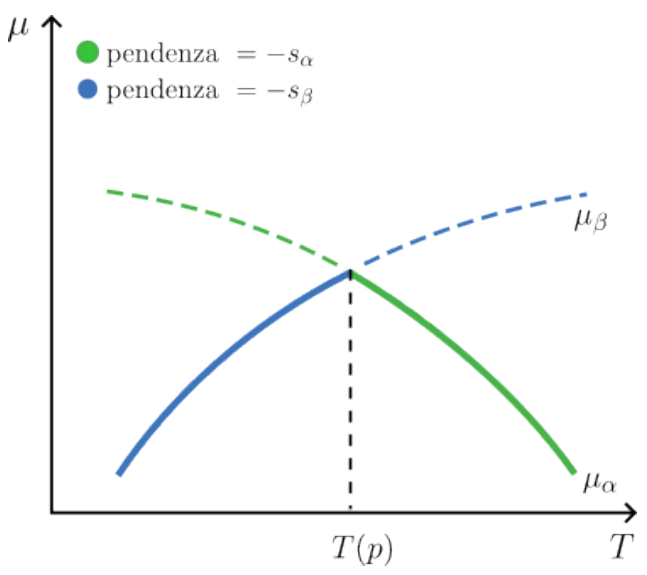
\includegraphics[width=0.4\linewidth]{Immagini/transizione I ordine p costante.png}
    \caption{transizione del primo ordine a pressione $p$ costante.}
    \label{fig: transizione I ordine p costante}
\end{figure}

Quindi, in generale alla transizione $S_\alpha \neq S_\beta$. In particolare, nell'esempio di sistema raffigurato in figura \ref{fig: transizione I ordine p costante}, si ha $S_\alpha > S_\beta$. Per $T = T(p) - \epsilon$, ossia subito prima della transizione, il sistema è nella fase $\beta$ per cui $S_{(-)} = NS_\beta$, invece per $T = T(p) + \epsilon$ il sistema è nella fase $\alpha$ per cui adesso $S_{(+)} = NS_\alpha$, dunque
\begin{equation}
    \Delta S = S_{(+)} - S_{(-)} = N(S_\alpha - S_\beta) > 0,
\end{equation}
cioè durante la transizione si ha un aumento di entropia e di conseguenza un calore latente $L$ dato da $L = T\Delta S$. Tale calore latente corrisponde anche alla variazione di entalpia del sistema, infatti se in
\begin{equation}
    H(S,p,N) = G(T,p,N) + TS
\end{equation}
si sostituisce la condizione di equilibrio $\mu_\alpha = \mu_\beta$, ossia $\Delta G = 0$, si ha
\begin{equation}
    \Delta H = \Delta(TS) = T\Delta S = L.
\end{equation}
Mantenendo invece costante la temperatura, la situazione tipica risulta essere simile a quella raffigurata in figura \ref{fig: transizione I ordine T costante}.
\begin{figure}[h]
    \centering
    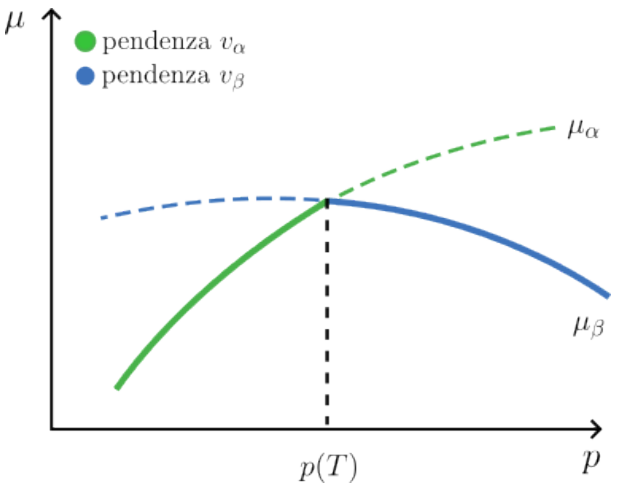
\includegraphics[width=0.4\linewidth]{Immagini/transizione I ordine T costante.png}
    \caption{transizione del primo ordine a temperatura $T$ costante.}
    \label{fig: transizione I ordine T costante}
\end{figure}

In generale, la derivata $\p_p\mu|_{T,N}$ è discontinua alla transizione. Siccome $\mu = G/N$ e $\p_pG|_{T,N} = V$ si ha, in una fase $\alpha$, che
\begin{equation}
    \frac{\p\mu_\alpha}{\p p}\bigg|_{T,N} = \frac{V_\alpha}{N_\alpha} = v_\alpha.
\end{equation}
Quindi, in generale alla transizione $v_\alpha \neq v_\beta$. In particolare, nell'esempio di sistema raffigurato in figura \ref{fig: transizione I ordine T costante}, si ha $v_\alpha > v_\beta$. Per $p = p(T) - \epsilon$, ossia subito prima della transizione, tutte le particelle sono nella fase $\alpha$ per cui $V_{(-)} = Nv_\alpha$, invece per $p = p(T) + \epsilon$ tutte le particelle sono nella fase $\beta$ per cui $V_{(+)} = Nv_\beta$, dunque
\begin{equation}
    \Delta V = V_{(+)} - V_{(-)} = N(v_\beta - v_\alpha) < 0.
\end{equation}
Quindi, se nella transizione si ha una discontinuità in
\begin{equation}
    \frac{\p\mu}{\p T}\bigg|_{p,N}\Longleftrightarrow\Delta S = \frac{L}{T}
\end{equation}
eventualmente insieme ad una discontinuità in
\begin{equation}
    \frac{\p\mu}{\p p}\bigg|_{T,N}\Longleftrightarrow\Delta V,
\end{equation}
la transizione è detta del ``primo ordine''.
\paragraph{Transizioni continue.} Se anche le derivate prime di $\mu$ sono continue alla transizione allora questa viene detta ``continua''. In tal caso, nella transizione stessa non si ha variazione di entropia né di volume, ossia $\Delta S = \Delta V = 0$. Vi sono però in generale discontinuità o singolarità in altre osservabili. Ad esempio, in un sistema con un solo tipo di componenti, una transizione continua può avvenire solo in punti nel piano $(p,T)$, detti ``punti critici'', che normalmente si trovano al termine di un tratto di una curva di coesistenza per una transizione del primo ordine. Il motivo di ciò è che in realtà esiste una richiesta di continuità aggiuntiva.

\section{Equazione di Clausius - Clapeyron}
Ci si chiede adesso come sia possibile determinare esplicitamente la curva di coesistenza $p(T)$ per una transizione del primo ordine. Per rispondere a ciò, si determina prima l'espressione per $dp/dT$ che poi, normalmente sotto qualche tipo di ipotesi semplificante, può essere integrata. Quindi, ricordando sempre che $\mu = G/N$ e che 
\begin{equation}
    d\mu = -sdT +vdp,\quad s = \frac{S}{N},\,v = \frac{V}{N},
\end{equation}
lungo la curva di coesistenza si ha $\mu_\alpha = \mu_\beta$, per cui spostandosi lungo essa di un tratto infinitesimo si ha $d\mu_\alpha = d\mu_\beta$, sostituendo ora l'espressione di $d\mu$ si ottiene
\begin{equation}
\label{eq: dp/dT per eq. CC}
    -s_\alpha dT + v_\alpha dp = -s_\beta dT + v_\beta dp,
\end{equation}
da cui, si ricava l'equazione di Clausius-Clapeyron
\begin{equation}
    \frac{dp}{dT} = \frac{\Delta S}{\Delta V},
\end{equation}
che può essere riscritta usando la relazione tra variazione di entropia e calore latente come
\begin{equation}
\label{eq: dp/dT per eq. CC in funzione di L}
    \frac{dp}{dT} = \frac{L}{T\Delta V} = \frac{l}{T\Delta v},\quad l =\frac{L}{N}.
\end{equation}
Siccome il membro di destra della \eqref{eq: dp/dT per eq. CC in funzione di L} è un rapporto, lo si può anche esprimere in termini del calore latente molare $l_{mol}$ e del volume molare $v_{mol}$ definiti come
\begin{equation}
    l_{mol} = \frac{L}{n_{mol}} = N_Al,\quad v_{mol} = \frac{V}{n_{mol}} = N_Av,
\end{equation}
oppure in termini del calore latente specifico $l_{spec}$ e del volume specifico $v_{spec}$, ossia riferiti all'unità di massa, definiti come
\begin{align}
    l_{spec} &= \frac{L}{M} = \frac{L}{n_{mol}m_{mol}} = \frac{l_{mol}}{m_{mol}}, \\
    v_{spec} &= \frac{V}{M} = \frac{V}{n_{mol}m_{mol}} = \frac{v_{mol}}{m_{mol}},
\end{align}
ottenendo dunque
\begin{equation}
    \frac{dp}{dT} = \frac{l_{mol}}{T\Delta v_{mol}} = \frac{l_{spec}}{T\Delta v_{spec}}.
\end{equation}

\subsubsection{Tensione di vapore saturo}
Come applicazione della relazione di Clausius - Clapeyron, si considera una transizione del primo ordine da liquido a gas, precisamente vapore. Quando le due fasi coesistono, e il vapore si dice ``saturo'', $p$ e $T$ sono sulla curva di coesistenza e vale l'equazione di Clausius - Clapeyron. Aumentando $T$ si passa dalla fase liquida o quella gassosa, il calore latente è positivo e per i volumi specifici si ha
\begin{equation}
    v_{gas} \gg v_{liquido}\quad\Rightarrow\quad \Delta v \sim \Delta v_{gas}.
\end{equation}
Dunque, l'equazione \eqref{eq: dp/dT per eq. CC in funzione di L} diventa
\begin{equation}
    \frac{dp}{dT} = \frac{l}{T\Delta v_{gas}}.
\end{equation}
Ipotizzando che il gas soddisfi l'equazione di stato dei gasi ideali $pv_{gas} = kT$ si ha
\begin{equation}
    \frac{dp}{dT} = \frac{lp}{kT^2}
\end{equation}
e supponendo anche che il calore latente sia costante lungo l'intero intervallo di temperatura considerato, si può integrare l'equazione trovata ora a variabili separabili ottenendo
\begin{equation}
    p(T) = p_0\exp{\bigg[-\frac{l}{k}\bigg(\frac{1}{T} - \frac{1}{T_0}\bigg)\bigg]}.
\end{equation}
Dunque, la pressione di vapore saturo cresce molto rapidamente in funzione della temperatura.

\section{Diagramma di fase nel piano (\textit{p,V})}
Considerando un sistema che esibisca una linea di transizione di fase del primo ordine nel piano $(p,T)$ ci si chiede ora come appaia tale diagramma di fase utilizzando invece le variabili coniugate $(p,V)$ per descrivere il sistema
\begin{figure}[h]
    \centering
    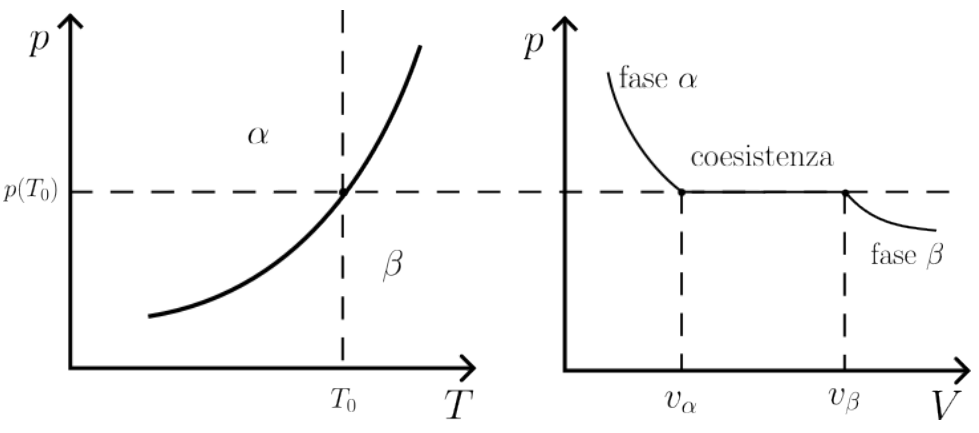
\includegraphics[width=0.6\linewidth]{Immagini/diagrammi p,T e p,V 1.png}
    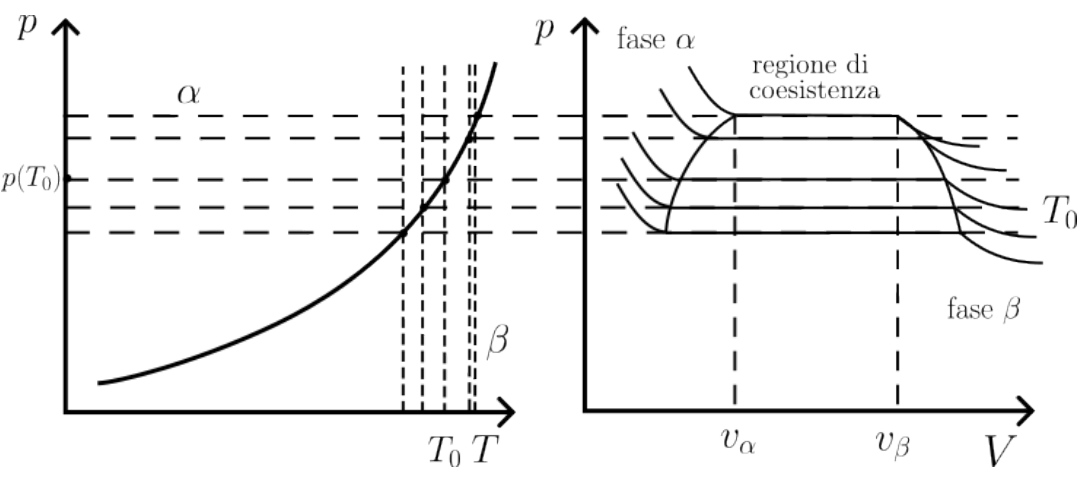
\includegraphics[width=0.6\linewidth]{Immagini/diagrammi p,T e p,V 2.png}
    \caption{relazione tra i piani $(p,T)$ e $(p,V)$.}
    \label{fig: diagrammi p,T e p,V}
\end{figure}
Facendo riferimento alla figura \ref{fig: diagrammi p,T e p,V}, il punto di transizione $(p(T_0),T_0)$ considerato diviene un segmento. Se si considerano le varie possibili isoterme si osserva che la singola curva di coesistenza diventa un'intera regione di coesistenza, dove si ricorda che la stabilità dello stato di equilibrio impone che
\begin{equation}
    \frac{\p p}{\p V}\bigg|_{T,N} \le 0,
\end{equation}
condizione soddisfatta dalle isoterme in figura \ref{fig: diagrammi p,T e p,V}. Adesso, si considera nuovamente un'isoterma fissata mostrata sempre in figura \ref{fig: diagrammi p,T e p,V}. Lungo il segmento orizzontale vi sono stati che differiscono per il numero di particelle $N_\alpha$ che sono nella fase $\alpha$ e quelli che sono nella fase $\beta$, il cui volume è
\begin{equation}
    V = N_\alpha v_\alpha + N_\beta v_\beta,\quad N_\beta = 1 - N_\alpha,
\end{equation}
che diviso per $N$, definendo $\nu_{\alpha,\beta} = N_{\alpha,\beta}/N$ restituisce il volume per particella 
\begin{equation}
\label{eq: volume spcifico}
    v = \nu_\alpha v_\alpha + \nu_\beta v_\beta,\quad \nu_\beta = 1 - \nu_\alpha.
\end{equation}
Da ciò seguono le relazioni
\begin{align}
    v - v_\alpha &= (\nu_\alpha - 1)v_\alpha + \nu_\beta v_\beta = -\nu_\beta v_\alpha + \nu_\beta v_\beta = \nu_\beta(v_\beta - v_\alpha), \\
    v_\beta - v &= -\nu_\alpha v_\alpha + (1 - \nu_\beta)v_\beta = -\nu_\alpha v_\alpha + \nu_\alpha v_\beta = \nu_\alpha(v_\beta - v_\alpha),
\end{align}
che divise membro a membro restituiscono la cosiddetta ``regola della leva''
\begin{equation}
\label{eq: regola della leva}
    \frac{\nu_\beta}{\nu_\alpha} = \frac{v - v_\alpha}{v_\beta - v}.
\end{equation}
I volumi specifici $v_\alpha$ e $v_\beta$ che determinano gli estremi del segmento di coesistenza nel grafico $p(v)$ ad una temperatura fissata $T$ sono implicitamente determinati dalle due condizioni
\begin{equation}
    \begin{cases}
        p_\alpha(T,v_\alpha) = p_\beta(T,v_\beta) = p(T) \\
        \mu_\alpha(T,v_\alpha) = \mu_\beta(T,v_\beta)
    \end{cases}.
\end{equation}
Di queste due condizioni si considera un'interpretazione geometrica in termini dell'energia libera di per particella $f = F/N$, l'energia libera di Helmoltz $F(T,V,N)$ in effetti è il potenziale rilevante quando le variabili indipendenti sono $T$, $V$ ed $N$. Siccome $p$ è data da
\begin{equation}
    -p = \frac{\p f}{\p v}\bigg|_{T,N},
\end{equation}
allora si può dedurre dal grafico di $p(v)$ quello di $f(v)$ per un valore di $T$ fissato. 
\begin{figure}[h]
    \centering
    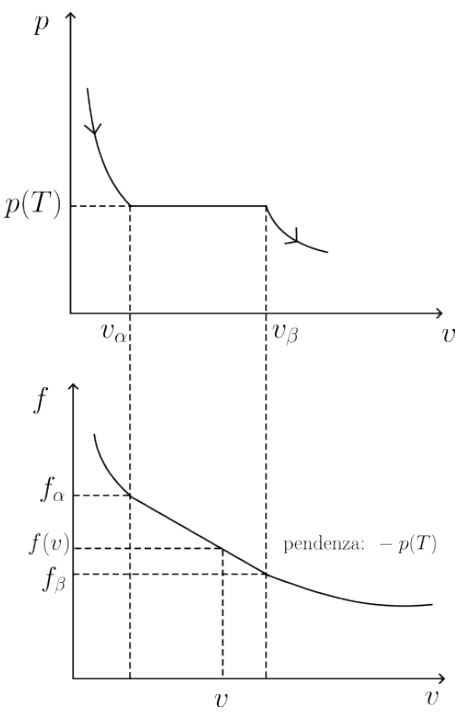
\includegraphics[width=0.45\linewidth]{Immagini/relazione digrammi p,v e f,v.png}
    \caption{relazione tra i piani $(p,v)$ e $(f,v)$.}
    \label{fig: relazione digrammi p,v e f,v}
\end{figure}

Ad esempio, si consideri il segmento rettilineo nel grafico \ref{fig: relazione digrammi p,v e f,v}, in questo caso si ha
\begin{equation}
    \begin{split}
        \frac{f_\beta - f_\alpha}{v_\beta - v_\alpha} &= -p \\
        f_\beta - f_\alpha &= -p(v_\beta - v_\alpha) \\
        (f + pv)_\beta &= (f + pv)_\alpha.
    \end{split}
\end{equation}
A causa della trasformata di Legendre che lega $F$ e $G$, $f + pv$ è l'energia di Gibbs specifica
\begin{equation}
    \mu = f + pv.
\end{equation}
Dunque, si è ritrovata la condizione $\mu_\alpha = \mu_\beta$. Per un generico $v\in[v_\alpha,v_\beta]$, come visto precedentemente, si ha $v = \nu_\alpha v_\alpha + \nu_\beta v_\beta$ quindi il valore di $f(v)$ desumibile dal grafico \ref{fig: relazione digrammi p,v e f,v}, cioè dalla proporzione
\begin{equation}
    \frac{f(v) - f_\alpha}{v - v_\alpha} = \frac{f_\beta - f_\alpha}{v_\beta - v_\alpha},
\end{equation}
che usando la relazione \eqref{eq: volume spcifico} diventa
\begin{equation}
    f = \nu_\alpha f_\alpha + \nu_\beta f_\beta.
\end{equation}

\section{Costruzione di Maxwell}
Si supponga di conoscere una descrizione approssimata di un certo sistema tramite un'equazione di stato $p \equiv p(T,V)$ che però, in alcune regioni, viola il criterio di stabilità, come ad esempio il caso del grafico in figura \ref{fig: costruzione di Maxwell}. In particolare, nella regione delimitata si ha la violazione
\begin{equation}
    \frac{\p p}{\p V}\bigg|_{T,N} > 0 \quad\Rightarrow\quad \kappa_T < 0.
\end{equation}
L'obiettivo quindi è rimpiazzare la curva contenuta nella regione compromessa con un'altra curva tale che:
\begin{enumerate}
    \item l'instabilità sia rimpiazzata da una transizione di fase del primo ordine che avviene ad una certa pressione $\bar{p}$;
    \item al di fuori della transizione l'equazione di stato rimanga quella graficata in figura \ref{fig: costruzione di Maxwell}.
\end{enumerate}
\begin{figure}[h]
    \centering
    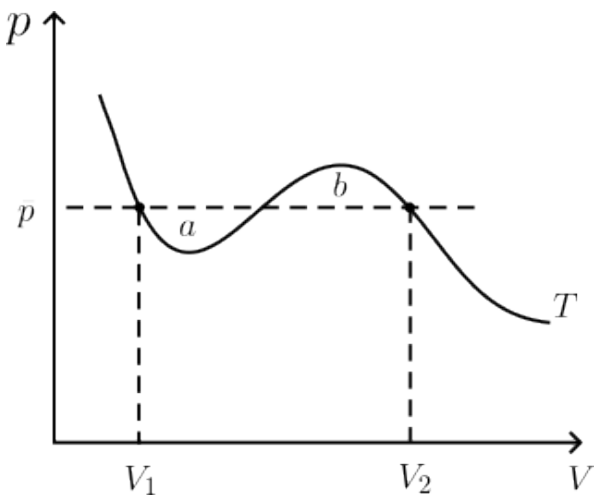
\includegraphics[width=0.4\linewidth]{Immagini/costruzione di Maxwell.png}
    \caption{costruzione di Maxwell per equazioni di stato violanti il criterio di stabilità.}
    \label{fig: costruzione di Maxwell}
\end{figure}

Essenzialmente, si vuole determinare il tratto orizzontale rappresentato in \ref{fig: costruzione di Maxwell} in modo che l'energia libera in $V_1$ e in $V_2$ coincida con quella prevista dall'equazione di stato approssimata. Siccome, l'energia libera $dF$ è data da
\begin{equation}
    dF = -SdT - pdV + \mu dN,
\end{equation}
ad $N$ e $T$ fissati si ha $dN = 0$ e $dT = 0$, per cui
\begin{equation}
    F(V_2,T,N) - F(V_1,T,N) = -\int_{V_1}^{V_2} p(V,T,N)\,dV.
\end{equation}
Se quest'ultimo integrale deve coincidere con la curva originale e per il segmento orizzontale, devono essere uguali le aree sottostanti. Quindi, $V_1$ e $V_2$ vanno determinati in modo che 
\begin{equation}
    \bar{p}(V_2 - V_1) = \int_{V_1}^{V_2} p(V,T)\,dV,
\end{equation}
dove $p(V,T)$ è la curva approssimata originale. In altri termini, le due aree indicate come $A$ e $B$ in figura \ref{fig: costruzione di Maxwell} devono risultare uguali. 

\subsection{Equazione di stato di Van der Waals}
L'equazione di stato di Van der Waals è un primo esempio di tentativo alla descrizione fenomenologica delle interazioni molecolari tra le componenti di un gas. Tipicamente, il potenziale intermolecolare ha una funzione del tipo graficato in figura \ref{fig: potenziale Van der Waals}. 
\begin{figure}[h]
    \centering
    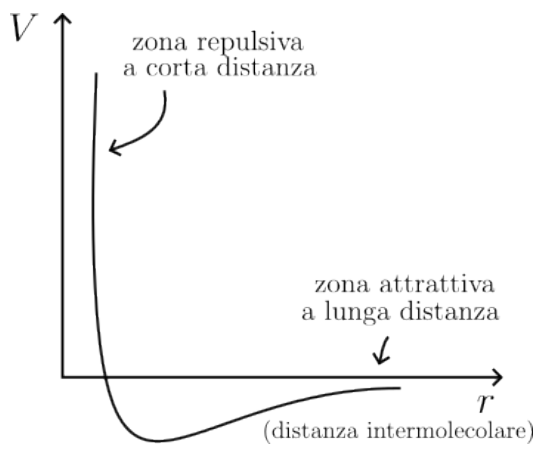
\includegraphics[width=0.4\linewidth]{Immagini/potenziale Van der Waals.png}
    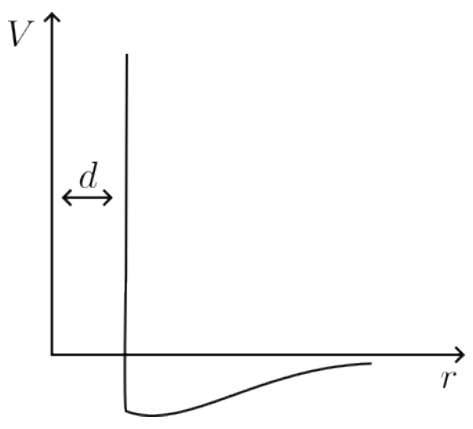
\includegraphics[width=0.36\linewidth]{Immagini/potenziale Van der Waals hardcore.png}
    \caption{(i) forma tipica del potenziale di interazione intermolecolare; (ii) approssimazione ``hardcore''.}
    \label{fig: potenziale Van der Waals}
\end{figure}

Il modello di Van der Waals descrive la regione repulsiva del potenziale tramite un ``hardcore'', ossia considerando le particelle come sfere indeformabili di un certo raggio, la conseguenza principale è che il volume effettivamente a disposizione delle molecole viene ridotto ad un volume efficace 
\begin{equation}
\label{eq: volume efficace Van der Waals}
    V_{eff} = V - b,\quad b\in\R
\end{equation}
dove $b$ è una costante che dipende unicamente dalla sostanza che compone il gas. La presenza di una parte attrattiva del potenziale implica la tendenza del sistema a formare stati legati. Questo comporta una diminuzione della pressione proporzionale al numero di coppie di molecole in uno stato vicino alle pareti. Questo effetto, è proporzionale al quadrato della densità $(N/V)^2$, quindi da
\begin{equation}
    \Delta p \propto n_{coppie} \propto \bigg(\frac{N}{V}\bigg)^2.
\end{equation}
L'ipotesi di Van der Waals è
\begin{equation}
\label{eq: I ipotesi Van der Waals}
    p = p_K - \frac{a}{V^2},
\end{equation}
dove $p_K$ è la pressione in assenza di interazioni ed è un'altra costante dipendente unicamente dalla sostanza in esame. Una ulteriore ipotesi è quella che $p_K$ soddisfi l'equazione di stato dei gas perfetti
\begin{equation}
\label{eq: II ipotesi Van der Waals}
    p_KV_{eff} = nRT.
\end{equation}
\begin{notz}
    D'ora in poi si considera il numero di moli $n$ pari a $n = 1$ in modo da non doverlo includere in ogni passaggio.
\end{notz}
Dunque, sostituendo le relazioni \eqref{eq: volume efficace Van der Waals} e \eqref{eq: I ipotesi Van der Waals} in \eqref{eq: II ipotesi Van der Waals} si ottiene l'equazione di stato di Van der Waals
\begin{equation}
\label{eq: equazione di stato Van der Waals}
    \bigg(p + \frac{a}{V^2}\bigg)(V - b) = RT.
\end{equation}
L'equazione \eqref{eq: equazione di stato Van der Waals} nel limite $V\to\infty$ si riduce all'equazione di stato classica dei gas perfetti $pV = RT$. In generale, l'equazione di Van der Waals è un polinomio di terzo grado in $V$, per cui un generico grafico delle isoterme è tipicamente del tipo rappresentato in figura \ref{fig: isoterme Van der Waals}. 
\begin{figure}[h]
    \centering
    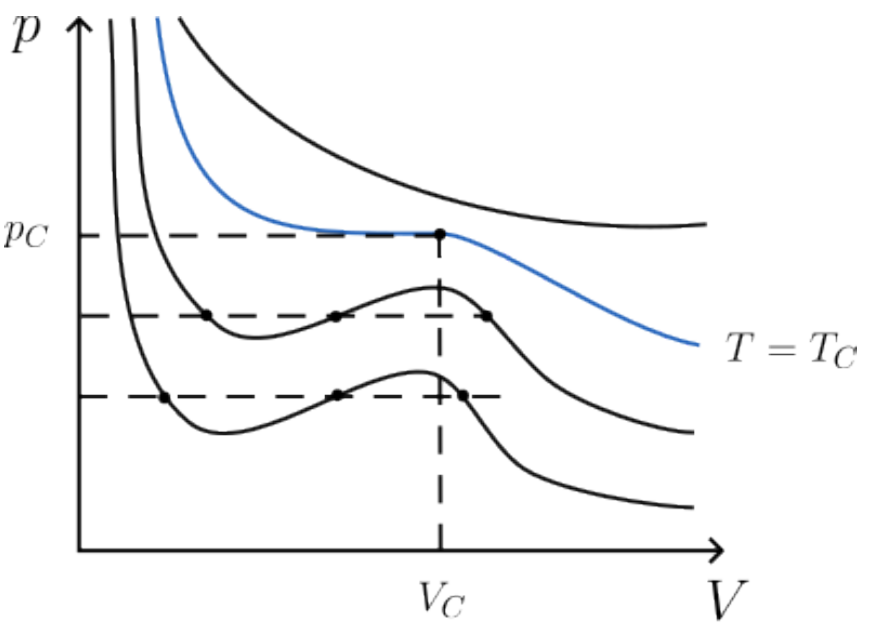
\includegraphics[width=0.42\linewidth]{Immagini/isoterme Van der Waals.png}
    \caption{grafico delle isoterme nel piano $(p,V)$ per l'equazione di Van der Waals.}
    \label{fig: isoterme Van der Waals}
\end{figure}

Tuttavia, al di sotto di una certa temperatura critica $T_C$ si nota che sarebbe comunque necessario usare la costruzione di Maxwell per correggere le previsioni dell'equazione \eqref{eq: equazione di stato Van der Waals}, la quale infatti trascura la possibilità di transizioni in cui il sistema si separa in due fasi. 
\begin{obs}
    L'equazione \eqref{eq: equazione di stato Van der Waals} si può parametrizzare invece che in termini di $a$ e $b$ che dipendono dalla sostanza in questione, in termini dei valori critici di pressione $p_C$, temperatura $T_C$ e volume $V_C$ indipendenti da essa. Definendo allora le variabili ridotte
    \begin{equation}
        \bar{p} = \frac{p}{p_C},\quad \bar{T} = \frac{T}{T_C},\quad \bar{V} = \frac{V}{V_C},
    \end{equation}
    si può esprimere l'equazione di stato di Van der Waals, dopo una serie di passaggi, come la ``legge degli stati corrispondenti'' 
    \begin{equation}
        \bigg(\bar{p} + \frac{3}{\bar{V}^2}\bigg)\bigg(\bar{V} - \frac{1}{3}\bigg) = \frac{8}{3}\bar{T}.
    \end{equation}
\end{obs}

\section{Coesistenza multifase}
Si considera una sistema con una singola componente che presenta al più tre fasi $\alpha$, $\beta$ e $\gamma$. La richiesta affinché queste fasi coesistano è
\begin{equation}
    \mu_\alpha(T,p) = \mu_\beta(T,p) = \mu_\gamma(T,p),
\end{equation}
che può essere ripartita in due equazioni indipendenti da $p$ e $T$
\begin{equation}
    \begin{cases}
        \mu_\alpha(T,p) = \mu_\gamma(T,p) \\
        \mu_\beta(T,p) = \mu_\gamma(T,p)
    \end{cases},
\end{equation}
la cui soluzione può essere un singolo punto o un insieme di punti. Un esempio, può essere il primo in figura \ref{fig: esempi di diagrammi di fase}, dove sono presenti due punti di coesistenza delle tre fasi, oppure il secondo sempre in figura \ref{fig: esempi di diagrammi di fase}, dove è presente un unico punto di coesistenza come accade per il diagramma di fase dell'acqua. 
\begin{figure}[h]
    \centering
    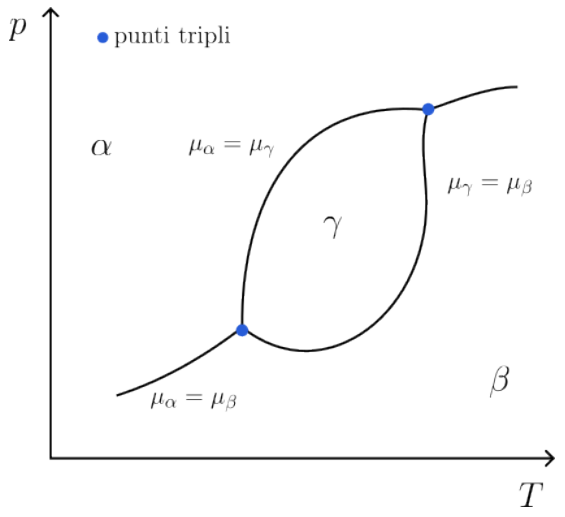
\includegraphics[width=0.4\linewidth]{Immagini/diagramma di fase (2 p.ti critici).png}
    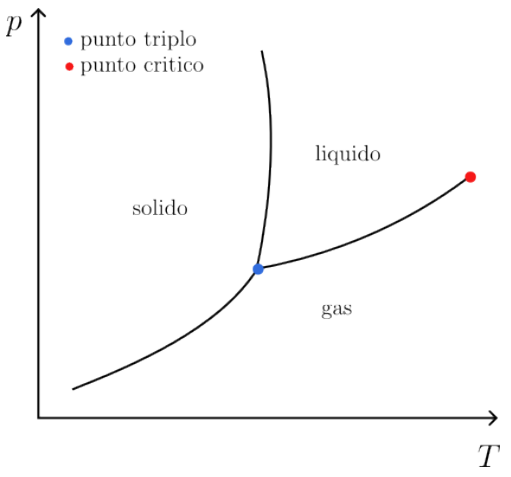
\includegraphics[width=0.39\linewidth]{Immagini/diagramma di fase (1 p.to critici).png}
    \caption{(ii) diagramma di fase fittizio con due punti critici; (ii) diagramma di fase dell'acqua.}
    \label{fig: esempi di diagrammi di fase}
\end{figure}

I punti di coesistenza vengono tipicamente chiamati ``punti tripli'', mentre agli estremi delle linee di transizione di fase possono essere presenti dei ``punti critici'' $C$. La presenza di tali punti critici, come nel caso dell'acqua, corrisponde, dal punto di vista qualitativo, che la fase liquida e la fase gassosa differiscono solo per un minore o un maggiore grado di interazione molecolare, permettendo di pensare di poter passare da uno all'altro senza dover passare da una linea di transizione. In altre parole, le transizioni oltre il punto critico le isoterme non presentano più alcuna transizione di fase del primo ordine e quindi le transizioni risultano essere continue, in particolare si ha $\Delta V = 0$. In pratica, si possono realmente distinguere le due fasi solo quando esistono contemporaneamente, cioè lungo la curva di coesistenza. 
\begin{obs}
    Ovviamente, un diagramma di fase può essere graficato su un piano differenze, ad esempio quello dell'acqua in figura \ref{fig: esempi di diagrammi di fase} sul piano $(p,T)$ può essere riportato invece su un piano $(p,V)$ come mostrato in figura \ref{fig: diagramma di fase acqua (p,V)}.
    \begin{figure}[h]
        \centering
        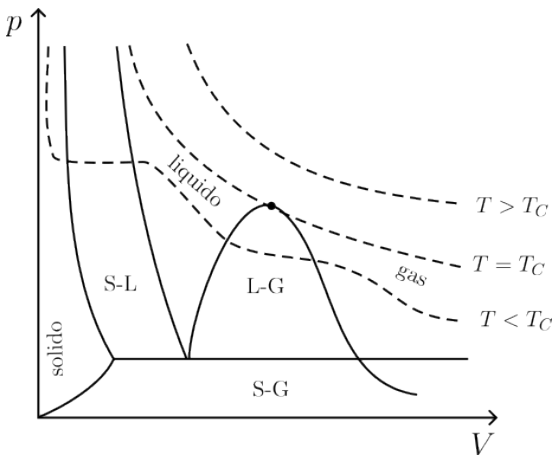
\includegraphics[width=0.4\linewidth]{Immagini/diagramma di fase acqua (p,V).png}
        \caption{diagramma di fase dell'acqua nel piano $(p,V)$.}
        \label{fig: diagramma di fase acqua (p,V)}
    \end{figure}
\end{obs}

\subsection{Sistemi multicomponenti}
Si supponga adesso di avere un sistema composto da una miscela di un certo numero $C$ di componenti macroscopiche diverse e che questo si trovi in una situazione di equilibrio in cui coesistono un certo numero $f$ di fasi. Si denota con $\nu_{i,a}$, con $i = 1,\dots,C$ e $\alpha=1,\dots,f$, la frazione di particelle dell'$i$-esimo tipo che si trovano nell'$\alpha$-esima fase, con la condizione che tali fasi debbano soddisfare il vincolo
\begin{equation}
    \nsum_i\nu_{i,\alpha} = 1,\quad\forall\alpha.
\end{equation}
Esistono quindi $(C - 1)$ variabili indipendenti per ogni $\alpha$, per un totale di $f(C - 1)$ variabili indipendenti. La condizione di coesistenza sono la costanza della coppia di variabili $(p,T)$ in tutte le fasi e l'uguaglianza dei potenziali chimici $\mu_{i,\alpha}$. Quindi, si hanno $C(f - 1)$ equazioni in $2 + f(C - 1)$ variabili
\begin{equation}
    \mu_{i,1}(p,T,\nu_{1,1},\dots,\nu_{C - 1,1}) = \cdots = \mu_{i,f}(p,T,\nu_{1,f},\dots,\nu_{C - 1,f}),\quad\forall i.
\end{equation}
Tutto ciò può essere interpretato come la coesistenza su una ipersuperficie parametrizzata da $2 + f(C - 1) - C(f - 1) = 2 + C - f$ variabili indipendenti. Dunque, il numero massimo di fasi $f$ coesistenti per un dato sistema di $C$ componenti è dato da
\begin{equation}
    f = 2 + C.
\end{equation}